\documentclass[tikz,border=8pt]{standalone}

\usepackage{amsmath}
\usepackage{bm}
\usetikzlibrary{arrows.meta,calc,positioning}

\begin{document}
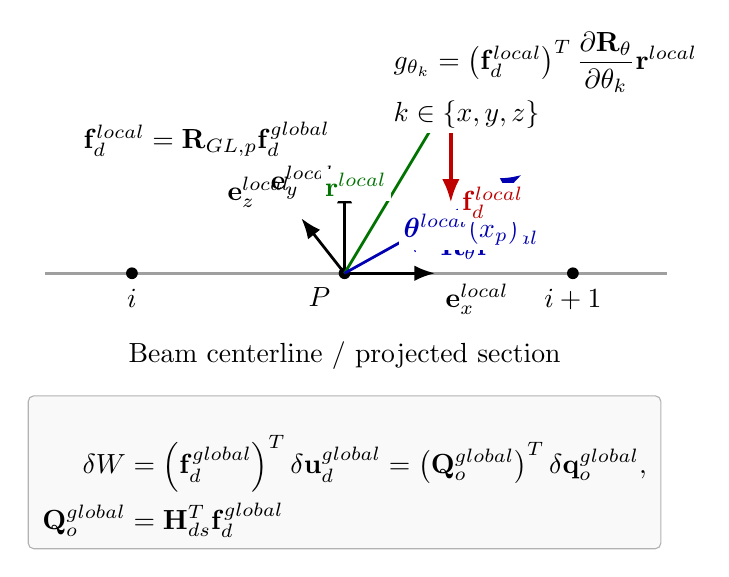
\begin{tikzpicture}[
    >=Latex,
    beam/.style={line width=1.1pt, gray!75},
    vector/.style={->, line width=1.0pt},
    force/.style={->, line width=1.2pt, red!75!black},
    rotated/.style={->, line width=1.0pt, blue!70!black},
    helper/.style={dashed, gray!65},
    point/.style={circle, fill=black, inner sep=1.5pt},
    labelbox/.style={fill=white, inner sep=1.5pt}
]

% Coordinates
\coordinate (A) at (-3.8,0.0);
\coordinate (B) at (4.1,0.0);
\coordinate (P) at (0.0,0.0);
\coordinate (Q) at (1.35,2.25);
\coordinate (Rdef) at (2.25,1.25);

% Beam centerline and nodes
\draw[beam] (A) -- (B);
\node[point, label=below:{$i$}] at (-2.7,0.0) {};
\node[point, label=below:{$i+1$}] at (2.9,0.0) {};
\node[point, label=below left:{$P$}] at (P) {};
\node[point, label=above right:{$Q$}] at (Q) {};

% Projection helper
\draw[helper] (Q) -- (P);
\draw[helper] (Q) -- ($(Q)!(P)!(B)$);

% Local frame at P
\draw[vector, black] (P) -- ++(1.15,0.0) node[below right] {$\mathbf{e}_x^{local}$};
\draw[vector, black] (P) -- ++(0.0,1.15) node[left] {$\mathbf{e}_y^{local}$};
\draw[vector, black] (P) -- ++(-0.55,0.7) node[above left] {$\mathbf{e}_z^{local}$};

% Offset and rotated offset
\draw[vector, green!45!black] (P) -- (Q)
    node[midway, left=2pt, labelbox] {$\mathbf{r}^{local}$};
\draw[rotated] (P) -- (Rdef)
    node[midway, below right=1pt, labelbox] {$\mathbf{R}_{\theta}\mathbf{r}^{local}$};

% Rotation indication
\draw[->, blue!70!black] (0.9,0.27) arc[start angle=18,end angle=32,radius=1.05];
\node[blue!70!black, labelbox] at (1.48,0.55) {$\boldsymbol{\theta}^{local}(x_p)$};

% Surface force
\draw[force] (Q) -- ++(0.0,-1.35)
    node[right=2pt, labelbox] {$\mathbf{f}_{d}^{local}$};

% Mapping annotations
\node[align=center, labelbox] at (-1.75,1.7)
    {$\mathbf{f}_{d}^{local}
      =\mathbf{R}_{GL,p}\mathbf{f}_{d}^{global}$};

\node[align=left, labelbox] at (2.55,2.45)
    {$g_{\theta_k}
      =
      \left(\mathbf{f}_{d}^{local}\right)^T
      \dfrac{\partial\mathbf{R}_{\theta}}{\partial\theta_k}
      \mathbf{r}^{local}$\\[2pt]
     $k\in\{x,y,z\}$};

\node[align=center, labelbox] at (0.0,-1.05)
    {Beam centerline / projected section};

% Conservative transfer summary
\node[draw=gray!60, rounded corners=2pt, align=left, fill=gray!5,
      text width=7.8cm, anchor=north] at (0,-1.55)
{
\begin{align*}
\delta W
&=
\left(\mathbf{f}_{d}^{global}\right)^T
\delta\mathbf{u}_{d}^{global}
=
\left(\mathbf{Q}_{o}^{global}\right)^T
\delta\mathbf{q}_{o}^{global},
\\
\mathbf{Q}_{o}^{global}
&=
\mathbf{H}_{ds}^{T}\mathbf{f}_{d}^{global}
\end{align*}
};

\end{tikzpicture}
\end{document}
